\def \secname {The Nonlinear Pendulum}

\section[\secname]{\hyperlink{toc}{\secname}}

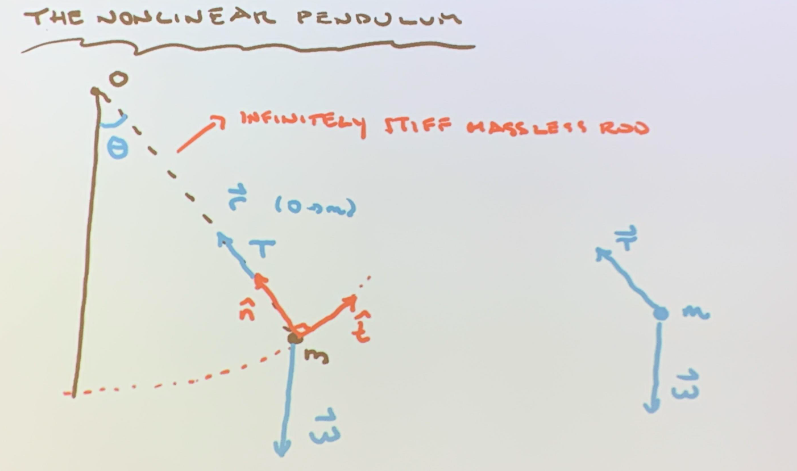
\includegraphics[width = 0.75 \linewidth]{Images/410_pendulumnonlinear.png}

\subsection{Physical and Mathematical Formulation}
\begin{itemize}
    \item Mass of Bob: m
    \item Infinetely rigid, massless pendulum arm; Length L $\equiv |\vec{r}|$
    \item No friction at pivot point. 0
    \item total mechanical energy (kinetic and potential) conserved
\end{itemize}
\subsubsection{Derivation of equation of motion}

\begin{itemize}
    \item Displacement vector $\vec{r}(t)$
    \item $\vec{r}(t)$ makes angle $
    \theta(t)$ (dynamical variable) with vertical
    \item Normal-tangential coordinate system, unit vectors; $\hat{n}$ and $\hat{t}$
    \item Velocity $\vec{v}(t)$ of Bob

    \[ \vec{v}(t) = \frac{d\vec{r}}{dt} = v \hat{t}\]
    \[ v \equiv |\vec{v}|\]

    Velocity is purely tangential
    
    \item Acceleration $\vec{a}(t)$

    \[ \vec{a}(t) = \frac{d^2\vec{r}}{dt^2} = \frac{d\vec{v}}{dt} = \frac{d}{dt} (v\hat{t}) = \frac{dv}{dt} \hat{t} + v \frac{d\hat{t}}{dt} = \frac{dv}{dt} \hat{t} + \frac{v^2}{L} \hat{n}\]

    Using $\frac{d\hat{t}}{dt} = \frac{v}{L} \hat{n}$ and fact that L is constant

    \item no motion in normal direction; consider only tangential motion
    \item tension force $\vec{T} = T \hat{n}$ and normal component of weight wcost irrelevant
    \item newton's 2nd law:

    \[ ma_t = F_t = -\omega \sin \theta = -mg \sin \theta \]

    where g is the acceleration due to gravity

    \[ a_t = -g \sin \theta \]

    \item rewrite as a function for $\theta (t)$

    \item angular velocity

    \[ \omega (t) = \frac{d\theta}{dt}\]

    \item Angular acceleration

    \[ \alpha(t) = \frac{d\omega}{dt} = \frac{d^2\theta}{dt^2}\]

    \[ L \alpha = a_t = L \frac{d^2\theta}{dt^2}\]

    \item sub in equation above and get:

    \[ \frac{d^2\theta}{dt^2} = -\frac{g}{L} \sin\theta \qquad 0 \leq t \leq t_{max}\]

    \item Need initial conditions

    \[ \theta(0) = \theta_0\]
    \[ \omega(0) = \omega_0\]

    these are specified values
\end{itemize}

\subsubsection{Non-dimensionalization}

\begin{itemize}
    \item Can change system of units so g=1, L=1, simplifies equation of motion; using \textbf{Natural Units} for problem.
    \item Adopting our new set of units, we want to solve is:

    \begin{equation}
        \frac{d^2\theta}{dt^2} = - \sin\theta \qquad 0 \leq t \leq t_{max}
    \end{equation}

    with initial conditions

    \begin{equation}
        \theta(0) = \theta_0
    \end{equation}

    \begin{equation}
        \omega(0) = \omega_0
    \end{equation}

    \item Equation above is nonlinear; can solve in closed form but the solution is complicated; FDA solution is no more complicated for a nonlinear case than for a linear case.
\end{itemize}

\subsubsection{Linear Limit}

\begin{itemize}
    \item Assume $\theta(t) \ll 1$

    \[ \sin \theta \approx \theta\]

    (3) $\rightarrow$

    \begin{equation}
        \frac{d^2\theta}{dt^2} = - \theta \qquad 0 \leq t \leq t_{max} 
    \end{equation}

    \item Has clenemal solution

    \[ \theta (t) = A \sin(t + \delta) \]

    where natural units, $\Omega \equiv 1$

    and $A, \delta $ determined by initial conditions

    \[ \Omega \equiv \sqrt{\frac{g}{L}} = 1 \]

    Independent of oscillation amplitude, A (equivalently independent of initial conditions)

    \item Not the case for the nonlinear pendulum
\end{itemize}

\subsection{Solution via FDA}

(HINT: serves as prototype for work in project 1)

Recall method:

\begin{itemize}
    \item Illustrates 3 key steps in solving ODEs (PDEs) with FDA
    \begin{enumerate}
        \item \textbf{Replace} Continuous Independent variable, t, with discrete values $0,\Delta t, 2\Delta t, 3\Delta t, ...$
        \item \textbf{Discretization of Equations: Replace derivatives with FDAs}
        \item \textbf{Solution:} Solve algebraic equations for approximate solution. Values (Here, once an initial condition x(0) is given)
    \end{enumerate}
\end{itemize}

Now Implement:

\subsubsection{Discretization: Step 1 - finite difference grid}

\begin{itemize}


    \item Continuous domain:
    \[ 0 \leq t \leq t_{max}\]

    \item Specify mesh via level parameter, l

    \[ n_t = 2^l + 1 \]

    \[ \Delta t = \frac{t_{max}}{n_t+1} = 2^{-l}t_{max}\]

    \[ t^n = (n-1) \Delta t, \qquad n=1,2,..., n_t\]
\end{itemize}

\subsubsection{Discretization Step 2 - Derivation of FDAs}

\begin{itemize}
    \item Continuum equations $\rightarrow$ Discrete Equations

    \[ \theta^n \equiv \theta (t^n) \equiv \theta ((n-1)\Delta t)\]
    

    \item One derivative to replace, use $O(\Delta t^2)$ centred approximation

    \begin{equation}
        \left. \frac{d^2 \theta}{dt^2} \right|_{t=t^n} \approx \frac{\theta^{n+1}-2\theta^n + \theta^{n-1}}{\Delta t^2}
    \end{equation}

    \begin{itemize}
        \item $t^{n+1}$
        \item $t^n \quad \rightarrow$ Centre-point for formula
        \item $t^{n-1}$
    \end{itemize}

    \item Should evaluate $\sin\theta$ at $t = t^n \quad \rightarrow \sin \theta^n$

    \item substituting in the equation above (27)

    \begin{equation}
        \frac{\theta^{n+1}-2\theta^n + \theta^{n-1}}{\Delta t^2} = -\sin\theta^n \qquad n+1 = 3,4,...,n_t
    \end{equation}
\end{itemize}


\textbf{Nonlinear pendulum (continued) September 29th 2023}

\begin{itemize}
    \item Sove for $\theta^{n+1}$
    \begin{equation}
        \theta^{n+1} = 2\theta ^n - \theta^{n-1} - \Delta t^2 \sin \theta^n \qquad n+1= 3,4,...,n_t
    \end{equation} 

    \item First discrete time we can use this, $t^{n+1} = t^3$

    \item Need value $\theta' = \theta(0)$; $\theta^2 = \theta(\Delta t)$ to initialize scheme 

    \item $\theta ' $ given by initial condition
    \[ \theta ' = \theta (0) = \theta_0\]

    \item $\theta^2 \rightarrow$ bit more involved; state without proof that we need $\theta^2$ to $O(\Delta t^3)$ accuracy so that overall solution is $O(\Delta t^2)$

    \item Heuristic justification: $t=t_{max}$ final time number of time steps is $\approx \frac{1}{\Delta t} = O(\Delta t^{-1})$. So per time step error needs to be $O(\Delta t^3)$ so that overall solution is $O(\Delta t^2)$

    \item Proceed via taylor series, use initial conditions 

    \[ \theta(\Delta t) = \theta (0) + \Delta t \frac{d\theta}{dt}(0) + \frac{1}{2} \Delta t^2 \frac{d^2\theta}{dt^2} (0) + O(\Delta t^3)\]

    \[ \approx \theta_0 + \Delta t \omega_0 + \frac{1}{2} \Delta t^2 \frac{d^2\theta}{dt^2}(0)\]

    Use equation of motion

    \[ = \theta_0 + \Delta t \omega_0 - \frac{1}{2} \Delta t^2 \sin\theta_0\]

    \item Assembling results

    \[ \theta^{n+1} = 2 \theta^n - \theta^{n-1} - \Delta t^2 \sin\theta^n \qquad n+1=3,4,...,n_t\]

    \[ \theta^1 = \theta_0\]

    \[ \theta^2 = \theta_0 + \Delta t \omega_0 - \frac{1}{2} \Delta t^2 \sin\theta_0\]

    \item Now have $n_t$ equations in $n_t$ unknowns and can solve.
\end{itemize}


\subsection{Convergence Analysis (error analysis)}

\begin{itemize}
    \item Want to examine behaviour of solution as $\Delta t \rightarrow 0$

    \item Assumption (Richardson, 1909) Let $U_*(t)$ be the exact (continuum) solution of some differential equation (example the equations above in example); then error is 

    \[ e(t^n) \equiv U_*(t^n) - U(t^n)\]

    Where $U(t^n)$ is the computed value

    \vspace{10px}

    And takes the form 

    \[ \lim_{\Delta t \rightarrow 0} e(t^n) = \Delta t^2 e_2(t^n) + O(\Delta t^4)\]

    where $e_2$ term is some function not some "random" error that would be seen in analyzing experimental data.
    \vspace{10px}
    note that order is 4 because the FDA is centred

    \item How do we know this?

    \item Deep question. Our approach: is to use it as an assumption for convergence analysis.
\end{itemize}

\subsubsection{Convergence Test}

Some mesh:
\[ o \qquad o \qquad o \qquad o \qquad o \qquad o \qquad o \qquad o \qquad o \qquad o \qquad o \qquad \]

\[ l, \Delta t_l, u_l^n\]

\[ o \quad o \quad o \quad o \quad o \quad o \quad o \quad o \quad o \quad o \quad o \quad \]

\[ l+1, \Delta t_{l+1} = \Delta t/2, u_{l+1}^n\]

\[ o \hspace{3 px} o \hspace{3 px} o \hspace{3 px} o \hspace{3 px} o \hspace{3 px} o \hspace{3 px} o \hspace{3 px} o \hspace{3 px} o \hspace{3 px} o \hspace{3 px} o \hspace{3 px} \]

\[ l+2, \Delta t_{l+2} = \Delta t/4, u_{l+2}^n\]

Always use at least 3 grids/ meshes, values of l
\begin{itemize}
    \item Then from equation above we have

    \[ u_l^n \approx u_*^n - (\Delta t_l)^2 e_2^n\]

    \[ u^n_{l+1} \approx u_*^n - (\Delta t_{l+1})^2 e_2^n\]

    \[ u^n_{l+2} \approx u_*^n - (\Delta t_{l+2})^2 e_2^n\]

    Think of n labelling common set of times (times on caorse gride l)

    \item Now subtract solutions on adjacent levels 

    \[ u_l^n-u_{l+1}^n \approx -((\Delta t_l)^2 - (\Delta t_{l+1})^2)e_2^n = \frac{-3}{4} \Delta t_l^2 e^n_2\]

     \[ u_{l+1}^n-u_{l+2}^n \approx - \frac{3}{4}((\Delta t_{l+1})^2 e_2^n = \frac{-3}{16} \Delta t^2_l e^n_2\]

     where the last term is error reduced by factor of 4

     \item Observation 

     \begin{enumerate}
         \item Get estimate of solution error by simply subtracting solutions on adjacent levels

         From equation earlier we have 

         \[ e^n = \Delta t^2 e_2^n + ...\]

         \[ u_l^n - u^n_{l+1} \approx -\frac{3}{4} (\Delta t_l)^2 l^n_2\]

         so 

         \[ -\frac{4}{3} (u_{l}^n - u_{l+1}^n) \approx e^n\]

         \item Consider the ratio

         \[ \frac{u^n_l - u^n_{l+1}}{u^n_{l+1} - u^n_{l+2}}\]

         in limit that $\Delta t_l \rightarrow 0$ should  get 

         \[ \frac{-(3/4)(\Delta t_l)^2 e_2^n}{-(3/16)(\Delta t_l)^2 e^n_2} = 4\]

         \item More useful in practice: scale (multiply) differences

         \[ u_l^n - u_{l+1}^n\ \text{by } 4^0=1\]
         \[ u_{l+1}^n - u_{l+2}^n\ \text{by } 4^1=4\]
         \[ u_{l+2}^n - u_{l+3}^n\ \text{by } 4^2=16\]

         And plot them (as a function of $t^n$) on single graph

         \vspace{10px}

         Curves should be nearly coincident and agreement should get better for higher levels

         \item Can use as many levels in the test as is feasible but use a minimum of 3

         \item \underline{Important}: don't have to know what the error is to do a convergence test

         \item \underline{Important}: If we don't observe convergence, good indication that we need to do some debugging.
     \end{enumerate}

\end{itemize}


\textbf{11:10am October 4th 2023}

\textbf{Energy Conservation}

Mechanical energy is conserved = use as check on implementation

\begin{itemize}

    \item For nonlinear pendulum

        \[ \text{kinetic energy} \equiv T(t) = \frac{1}{2} mv(t)^2 = \frac{1}{2} m (L \omega (t))^2\]

        \[ \text{potential energy} \equiv V(t) = mgh(t)\]

        where h(t) is vertical displacement of bob from equilibrium height

        \[ \text{total energy} = E(t) = T(t) + V(t)\]

        
    \[ \text{Total Energy } = E(t) = T(t) + V(t) \]

    \[ E(t) = \frac{1}{2} m (L\omega(t))^2 + mgL(1-\cos\theta(t))\]

    
    \item Our units: g=1, L=1, m=1 (MLT)

    \[ E(t) = T(t) + v(t) = \frac{1}{2} \omega (t)^2 + (1-\cos\theta(t)\]

    \item Track deviation in energy 
    \[ dE(t) \equiv E(t)-E(0)\]

    \item One thing to do: plot it and see whether it "Looks Good"

    \item Better: Check convergence of $dE(t;\Delta t)$

    \[ \Rightarrow \text{Expect} \qquad dE(t; \Delta t) = \Delta t^2 \epsilon(t) + ... \qquad \text{Where epsilon is some function}\]

    \[ \Rightarrow \text{As } \Delta t \rightarrow 0 \qquad dE(t;\Delta t) \rightarrow 0 \text{ As } \Delta t^2\]

    \[ \Rightarrow \text{Plot } \quad dE(t; \Delta t), 4dE(t; \Delta t/2), 16 dE(t; \Delta t/4), ...\]

    Should be neatly coincident

    \item Calculations should display convergence to conservation

    \item For \textbf{linear} pendulum need another expression for total energy
    \item Small angle approximation

    \[ \cos\theta = 1 - \frac{1}{2} \theta ^2 + O(\theta^4) \approx 1- \frac{1}{2}\theta^2\]

    \[ \Rightarrow E_{Linear}(t) = T(t) + V(t) = \frac{1}{2}\omega(t)^2 + \frac{1}{2} \theta (t)^2\]
    
\end{itemize}

\textbf{End of FDA discussion - will use convergence testing and FDA lots in projects and HW!}
